\subsection{Model}
\verbatiminput{alloy.als}

\subsection{Alloy result}
	The model is consistent: see Figure 4.
	\begin{figure}
		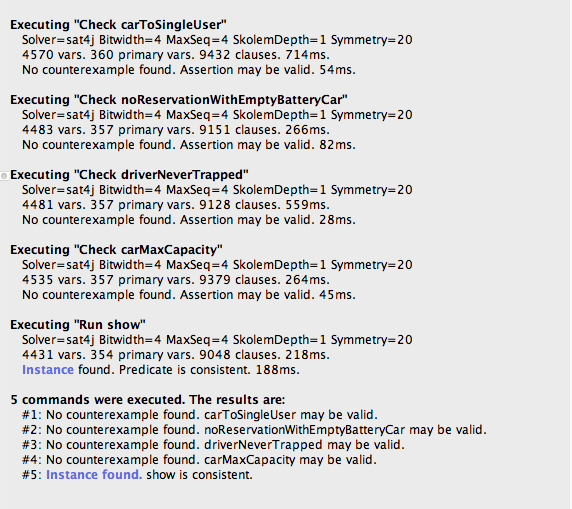
\includegraphics[width=\textwidth]{img/alloy_output.png}
		\caption{Result of the model analysis.}
		\label{figure 1}
	\end{figure}



	\begin{landscape}
	
	\subsection{Worlds generated}
	
		\subsubsection{General world}
			\begin{figure}				
				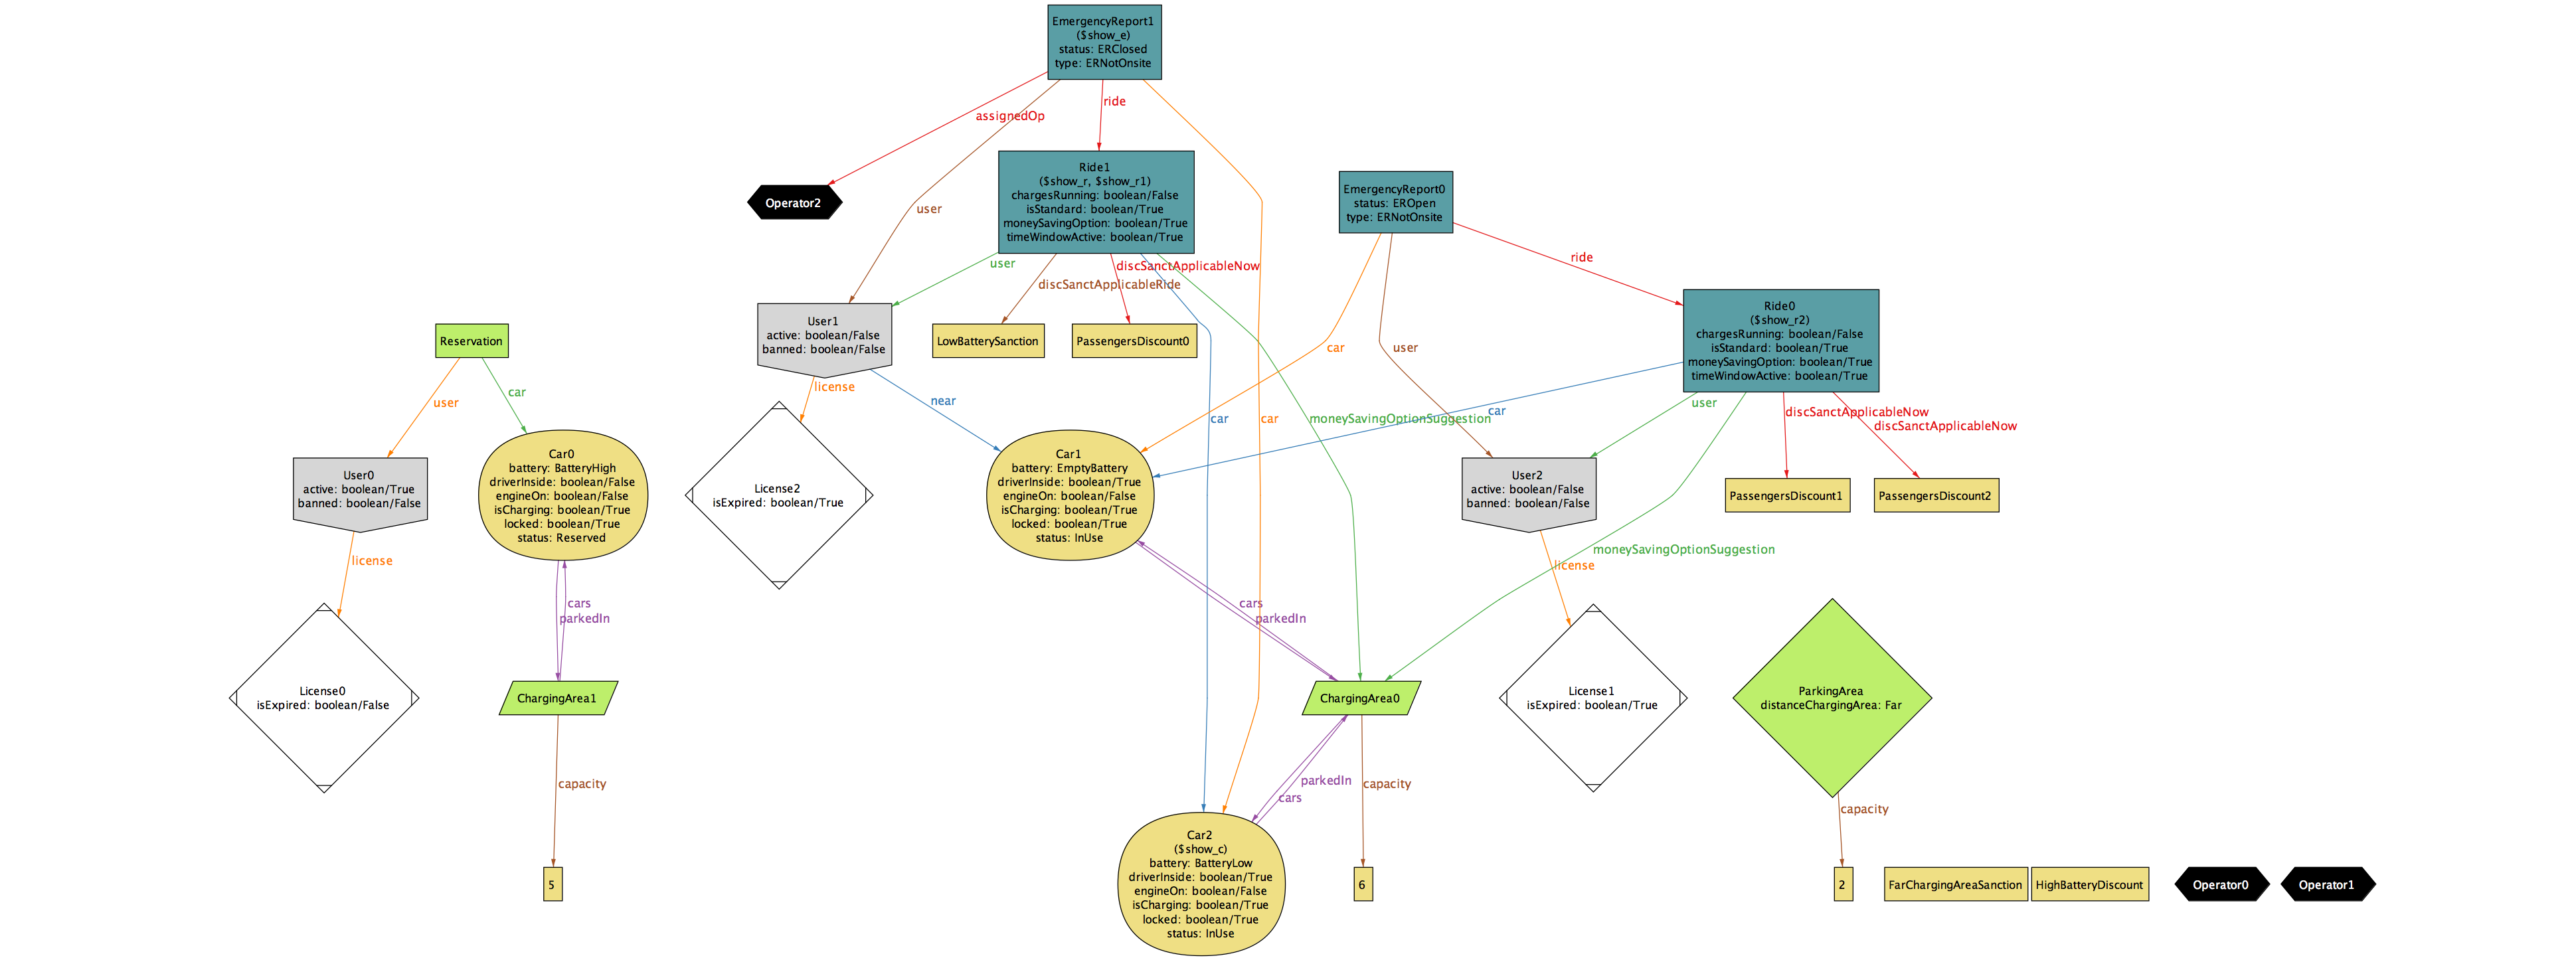
\includegraphics[width=2\textwidth, center]{img/world1.png}
				\caption{World generated.}
				\label{figure 1}
			\end{figure}
	
		\subsubsection{Ride-reservation projection}
			\begin{figure}						
				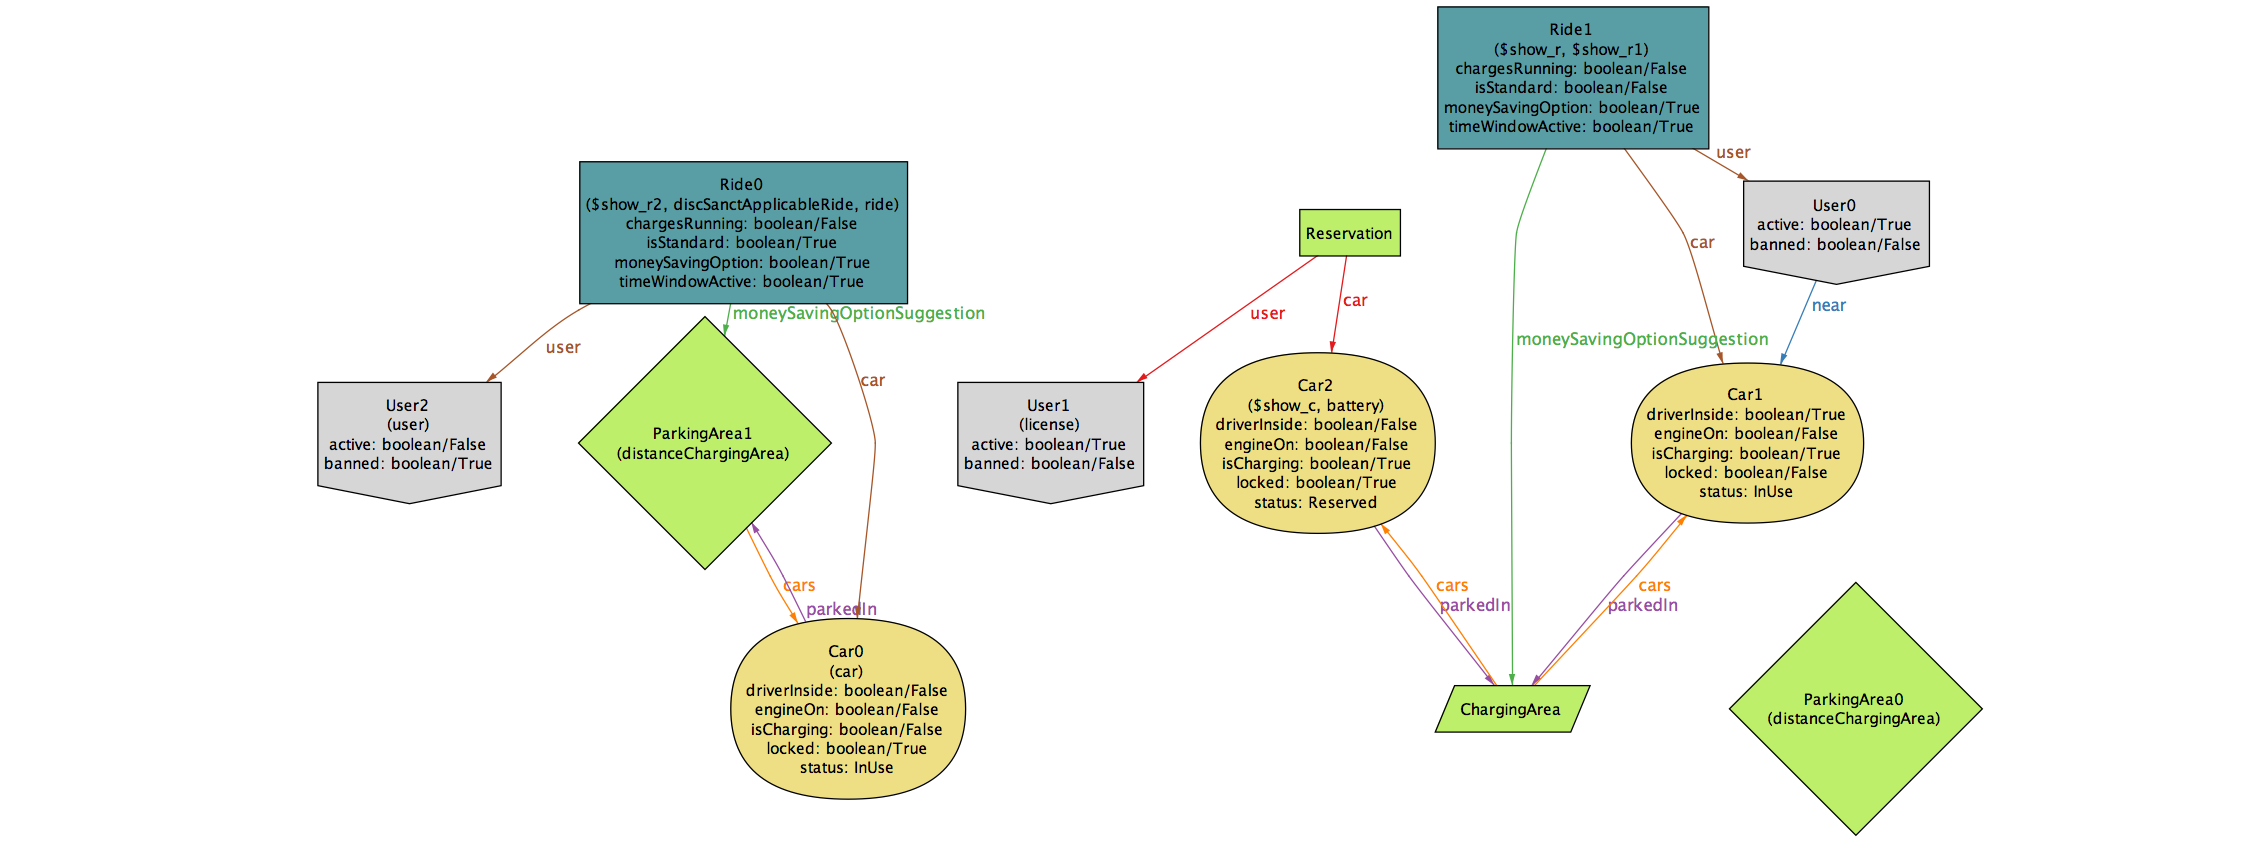
\includegraphics[width=2\textwidth, center]{img/rides_reservations.png}
				\caption{Ride-reservation projection.}
				\label{figure 2}
			\end{figure}

	
		\subsubsection{User licenses projection}
			\begin{figure}	
				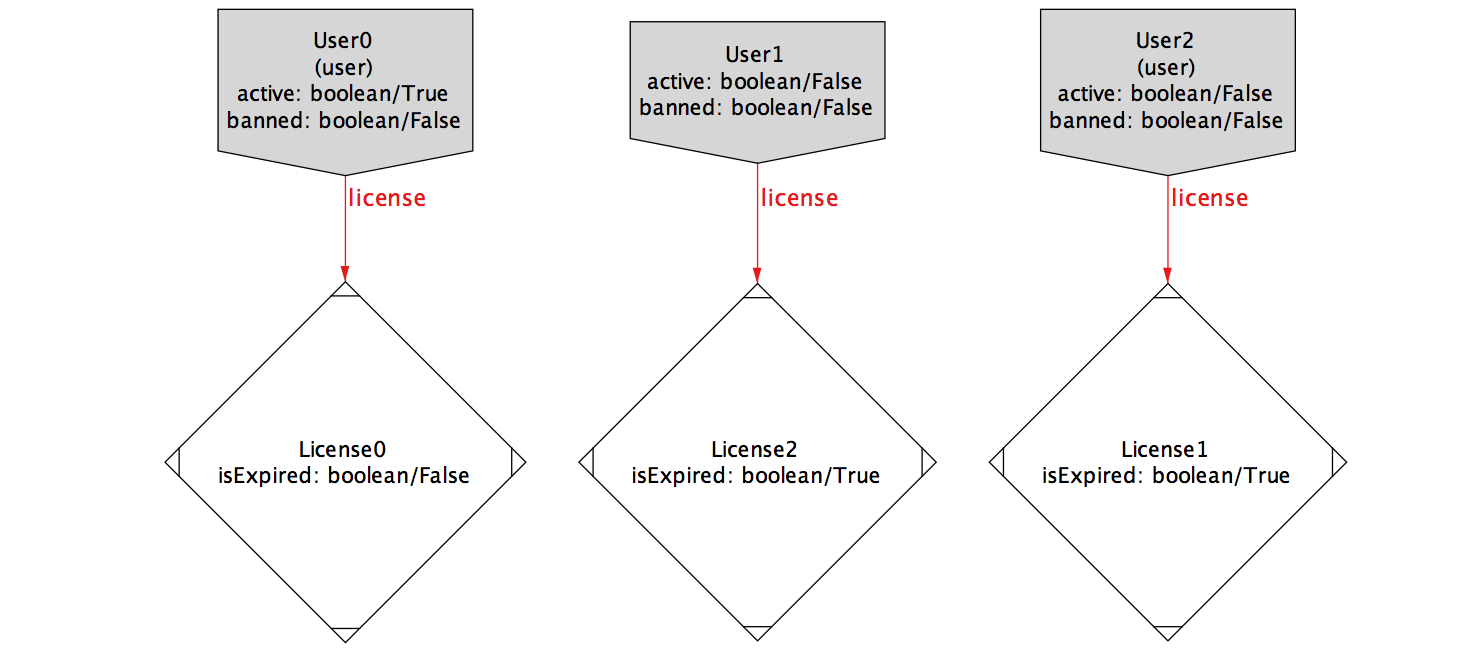
\includegraphics[width=2\textwidth, center]{img/user_licenses.png}
				\caption{User licenses projection.}
				\label{figure 3}
			\end{figure}
		
		\subsubsection{Emergency report projection}
			\begin{figure}	
				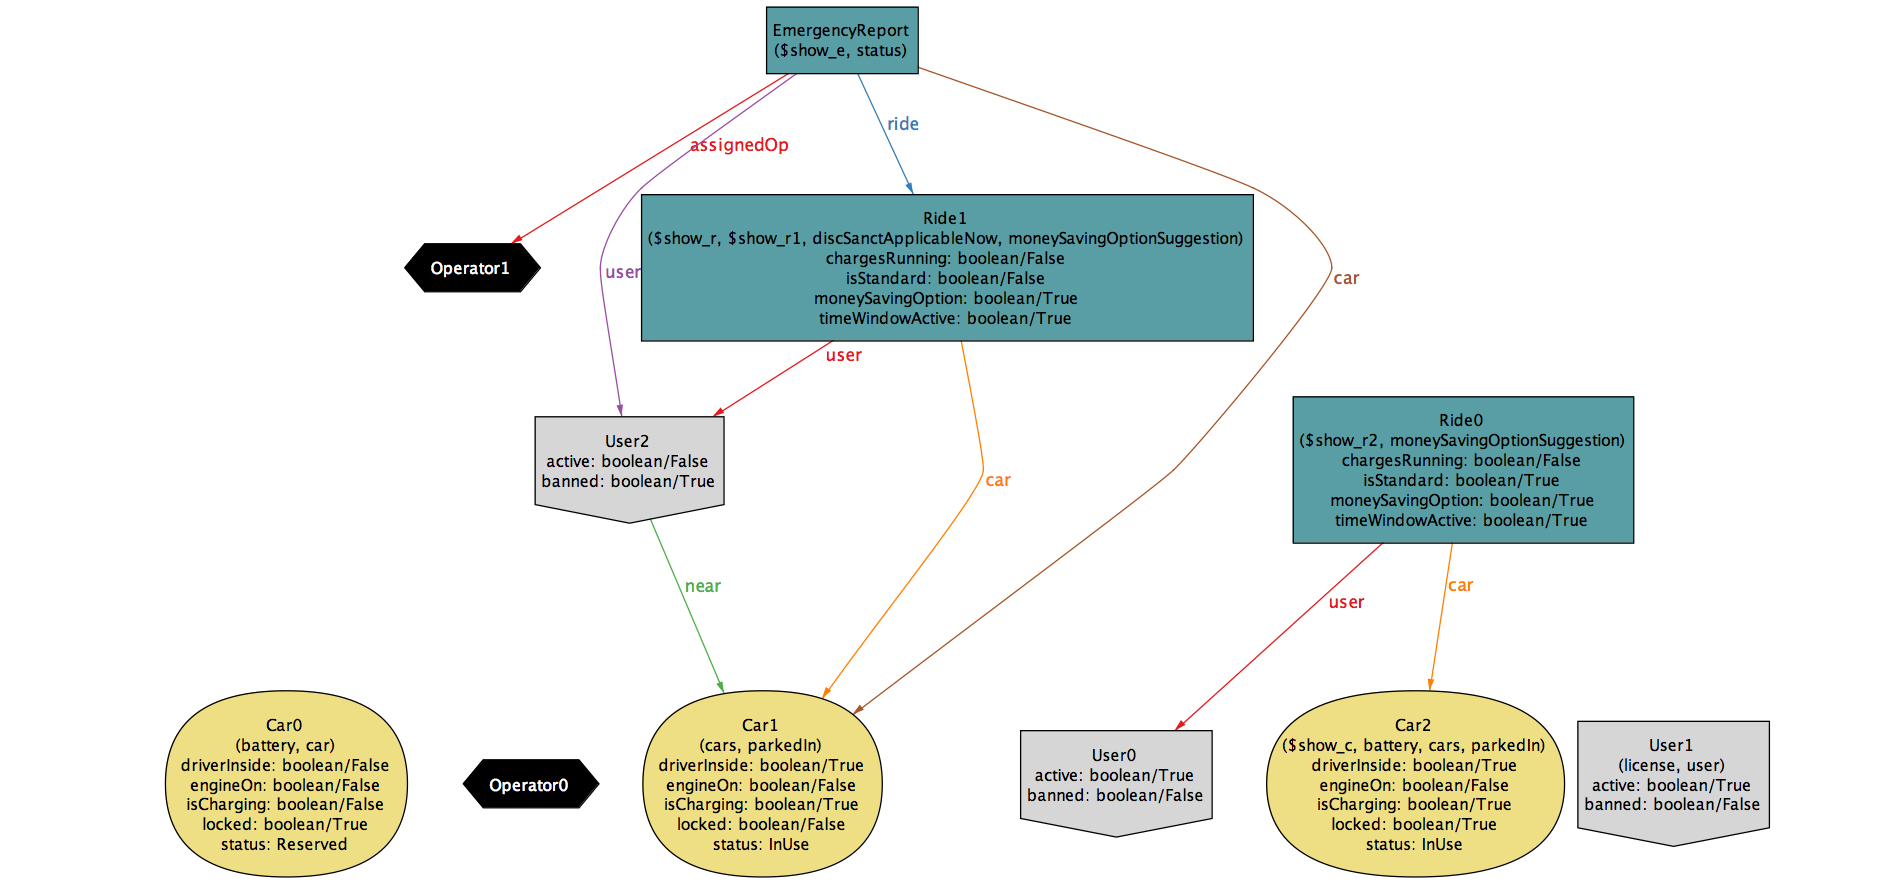
\includegraphics[width=2\textwidth, center]{img/emergency_reports.png}
				\caption{User licenses projection.}
				\label{figure 3}
			\end{figure}
	
	\subsection{Metamodel}
	\end{landscape}